\documentclass[aspectratio=169]{beamer}
\usepackage{tikz}
\usepackage{graphicx}
\usepackage{listings}
\usepackage{xcolor}
\usepackage{hyperref}
\usepackage[spanish,es-noquoting]{babel}
\usepackage[round]{natbib}

\lstset{
  basicstyle=\ttfamily\small,
  keywordstyle=\color{blue},
  stringstyle=\color{red},
  commentstyle=\color{gray},
  showstringspaces=false
}

% Clean Theme Setup & Optimization
\usetheme{Warsaw}
\usecolortheme{default}
\usefonttheme{serif}

% Remove top headline bar and navigation clutter to maximize slide text space
\setbeamertemplate{headline}{}
\setbeamertemplate{navigation symbols}{}
\setbeamertemplate{frametitle continuation}{}

% Slim, clean footline bar
\setbeamertemplate{footline}{
  \leavevmode%
  \hbox{%
    \begin{beamercolorbox}[wd=.333333\paperwidth,ht=2.25ex,dp=1ex,left]{author in head/foot}%
      \hspace*{2ex}\insertshortauthor
    \end{beamercolorbox}%
    \begin{beamercolorbox}[wd=.333333\paperwidth,ht=2.25ex,dp=1ex,center]{title in head/foot}%
      \insertshorttitle
    \end{beamercolorbox}%
    \begin{beamercolorbox}[wd=.333333\paperwidth,ht=2.25ex,dp=1ex,right]{date in head/foot}%
      \insertframenumber{} / \inserttotalframenumber\hspace*{2ex}
    \end{beamercolorbox}%
  }%
  \vskip0pt%
}

% Font size and list spacing optimizations to prevent text overflow
\setbeamertemplate{itemize/enumerate body begin}{\small}
\setbeamertemplate{itemize/enumerate subbody begin}{\footnotesize}
\setbeamertemplate{itemize/enumerate subsubbody begin}{\scriptsize}

\makeatletter
\g@addto@macro\itemize{%
  \setlength{\itemsep}{2pt}%
  \setlength{\parsep}{1pt}%
  \setlength{\topsep}{2pt}%
  \setlength{\partopsep}{0pt}%
}
\makeatother

\graphicspath{{../}{./}}
\setbeamertemplate{caption}[numbered]

% Title info
\title[ IA y Derecho]{ IA y Derecho: Todo lo que necesitas saber antes de empezar}
\subtitle{ De Modelos Fundacionales a Estrategia Legal (Módulo 1)}
\author{Ricardo Reyes-Jimenez}
\institute{Universidad de La Sabana}
\date{\today}


% Background image for title slide
\usebackgroundtemplate{
  \tikz\node[opacity=0.3]{
\includegraphics[width=\paperwidth,height=\paperheight]{Images/UniSabana.jpg}};
}


\begin{document}

% Title slide
\begin{frame}
  \titlepage
\end{frame}

% Reset background for normal slides
\usebackgroundtemplate{}


\begin{frame}[allowframebreaks,fragile]{Objetivos de la Sesión}


\begin{itemize}
  \item Entender la arquitectura tecnológica moderna (2026): IA Generativa vs Tradicional.
  \item Orquestación: Por qué las plataformas legales usan múltiples modelos a la vez.
  \item Adopción real: Qué funciona hoy en Colombia y el mundo.
  \item Casos de uso inmediatos y herramientas clave (Harvey, Lexis+AI, Claude, etc.).
  \item Gestión de Riesgos: Privacidad y Propiedad Intelectual.
\end{itemize}
\end{frame}

\begin{frame}[allowframebreaks,fragile]{Desmitificando la Tecnología (El ``Matryoshka'' de la IA)}


\textbf{Conceptos Fundamentales:}

\begin{itemize}
  \item \textbf{Inteligencia Artificial (IA):} Máquinas replicando capacidades cognitivas.
  \item \textbf{Machine Learning \& Deep Learning:} Aprendizaje a partir de datos históricos mediante redes neuronales.
  \item \textbf{IA Generativa y LLMs (Large Language Models):} Modelos estadísticos avanzados que predicen lenguaje. No ``piensan'' como abogados, calculan probabilidades semánticas.
\end{itemize}
\end{frame}

\begin{frame}[allowframebreaks,fragile]{El ``Matryoshka'' de la IA (Visual)}


\begin{figure}\centering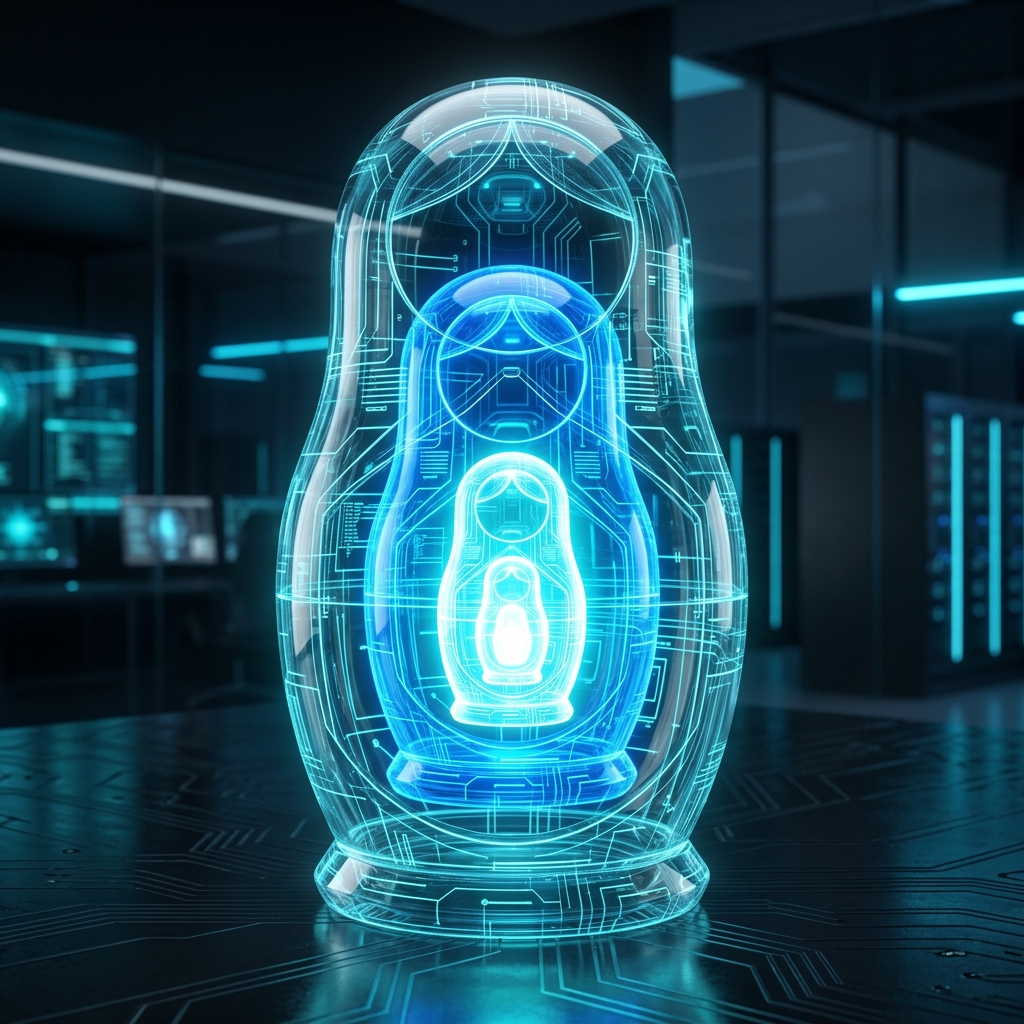
\includegraphics[height=0.6\textheight,keepaspectratio]{Images/matryoshka_ai_1785900912673.png}\caption{Matryoshka de la IA}\end{figure}

\end{frame}

\begin{frame}[allowframebreaks,fragile]{Evolución 2026: De Modelos Solos a Sistemas Orquestados}


\textbf{¿Cómo funciona una plataforma LegalTech de alto nivel (ej. Harvey o Lexis+AI)?}

\begin{itemize}
  \item \textbf{No es un solo modelo:} No le hablan a un único 'cerebro'.
  \item \textbf{Sistemas Multi-Modelo:} Hay un modelo que lee tu pregunta (Router), otro especializado en extraer leyes, otro en razonar el caso, y otro que redacta el texto final.
  \item \textbf{RAG (Generación Aumentada por Recuperación):} La IA consulta la base de datos de jurisprudencia de la firma \textit{antes} de responder, eliminando alucinaciones \cite{relativity2024}.
\end{itemize}
\end{frame}

\begin{frame}[allowframebreaks,fragile]{Automatización vs. Inteligencia Artificial}


\textbf{El Cambio en el Despacho}

\begin{itemize}
  \item \textbf{RPA (Tradicional):} Macros, flujos rígidos. (\texttt{SI A $\rightarrow$ ENTONCES B}). Falla si el documento cambia.
  \item \textbf{IA Generativa:} Interpreta contexto. Puede leer un correo furioso, entender la intención, y redactar una respuesta conciliatoria.
\end{itemize}
\end{frame}

\begin{frame}[allowframebreaks,fragile]{RPA vs IA Generativa (Visual)}


\begin{figure}\centering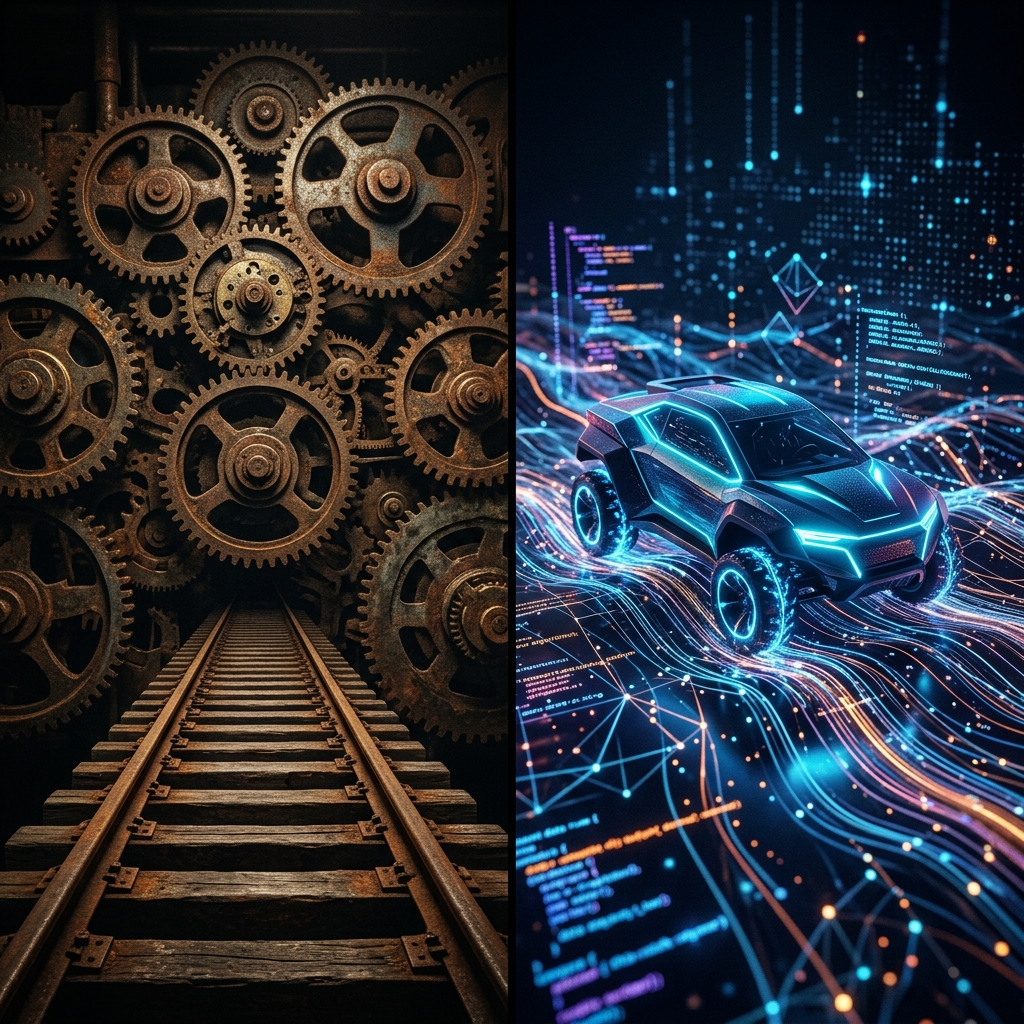
\includegraphics[height=0.6\textheight,keepaspectratio]{Images/rpa_vs_genai_1785900922553.png}\caption{RPA vs IA Generativa}\end{figure}

\end{frame}

\begin{frame}[allowframebreaks,fragile]{Ejercicio Plenario: ¿RPA o IA Generativa?}


\textbf{Analicemos las siguientes tareas. ¿Qué tecnología usaría?}

\begin{itemize}
  \item \textbf{Caso 1:} Enviar un correo estándar de cobro pre-redactado cada vez que una factura vence en el sistema contable. \textit{(¿RPA o IA?)}
  \item \textbf{Caso 2:} Leer un contrato de arrendamiento de 50 páginas y extraer un resumen de las obligaciones del arrendatario. \textit{(¿RPA o IA?)}
  \item \textbf{Caso 3:} Descargar los estados judiciales diarios, buscar el nombre de la firma y guardarlos en una carpeta específica. \textit{(¿RPA o IA?)}
  \item \textbf{Caso 4:} Recibir un correo de un cliente muy molesto, interpretar su tono y redactar una propuesta de respuesta conciliatoria. \textit{(¿RPA o IA?)}
\end{itemize}
\end{frame}

\begin{frame}[allowframebreaks,fragile]{Casos de Uso de Alto Impacto y Herramientas (2026)}



\begin{table}
\resizebox{\textwidth}{!}{
\begin{tabular}{|l | l | l | l|}
\hline
\textbf{Herramienta} & \textbf{Caso de Uso Principal} & \textbf{Sitio Web} & \textbf{Referencia} \\ \hline
Harvey AI & Investigación y Análisis Complejo & \href{https://www.harvey.ai/}{harvey.ai} & \cite{harvey2024} \\ \hline
Lexis+ AI & Investigación Jurídica y Jurisprudencia & \href{https://www.lexisnexis.com/en-us/products/lexis-plus-ai.page}{lexisnexis.com} & \cite{lexis2024} \\ \hline
Luminance & Due Diligence y Revisión de Contratos & \href{https://www.luminance.com}{luminance.com} & \cite{luminance2024} \\ \hline
vLex & Inteligencia Legal Global y Derecho Comparado & \href{https://vlex.com}{vlex.com} & \cite{vlex2024} \\ \hline
CoCounsel & Asistente Legal Integrado (Casetext/TR) & \href{https://legal.thomsonreuters.com/en/casetext}{casetext.com} & \cite{cocounsel2024} \\ \hline
Spellbook & Redacción y Revisión en Microsoft Word & \href{https://www.spellbook.legal}{spellbook.legal} & \cite{spellbook2024} \\ \hline
Clearbrief & Verificación de Hechos y Escritos Judiciales & \href{https://clearbrief.com}{clearbrief.com} & \cite{clearbrief2024} \\ \hline
Relativity aiR & E-Discovery y Revisión Documental Masiva & \href{https://www.relativity.com/data-solutions/ai/}{relativity.com} & \cite{relativityair2024} \\ \hline
Everlaw & Gestión de Litigios e Investigaciones & \href{https://www.everlaw.com}{everlaw.com} & \cite{everlaw2024} \\ \hline
Ironclad AI & Gestión del Ciclo de Vida de Contratos (CLM) & \href{https://ironcladapp.com}{ironcladapp.com} & \cite{ironclad2024} \\ \hline
Sof-IA (Sophia) & Asistente Inteligente (Tirant lo Blanch) & \href{https://tirant.com}{tirant.com} & \cite{tirant2024} \\ \hline
Juztina & Asistente de Investigación para LatAm & \href{https://www.juztina.ai}{juztina.ai} & \cite{juztina2024} \\ \hline
silvIA & Asistente Legal Especializado (LEGIS) & \href{https://www.legis.com.co}{legis.com.co} & \cite{legis2024} \\ \hline
\end{tabular}
}
\end{table}
\end{frame}

\begin{frame}[allowframebreaks,fragile]{Adopción Real: Colombia y el Resto del Mundo}


\begin{itemize}
  \item \textbf{Tendencia Global:} Las firmas ya no evalúan `\texttt{si'' usar IA, sino }`cómo'' integrarla en flujos (Word, Teams) y medir el ROI \cite{thomsonreuters2024}.
  \item \textbf{Colombia / LatAm:} Transición de pilotos a infraestructura base. Los clientes empiezan a exigir eficiencias basadas en IA en la facturación (Adiós al modelo de horas facturables en tareas repetitivas).
\end{itemize}
\end{frame}

\begin{frame}[allowframebreaks,fragile]{El Dilema Estratégico: Construir vs. Comprar (Build vs. Buy)}


\begin{itemize}
  \item \textbf{Comprar (Licenciar):} Herramientas listas para usar (Harvey, Lexis+ AI).
  \begin{itemize}
    \item \textit{Pros:} Implementación rápida, infraestructura mantenida por el proveedor.
    \item \textit{Contras:} Alto costo de licenciamiento, dependencia del vendedor.
  \end{itemize}
  \item \textbf{Construir (In-House):} Usar APIs (OpenAI, Anthropic) para crear un entorno propio (Azure/AWS).
  \begin{itemize}
    \item \textit{Pros:} Control total de datos, personalización profunda, menor costo variable a largo plazo.
    \item \textit{Contras:} Requiere equipo de ingeniería, mantenimiento constante y gestión de infraestructura.
  \end{itemize}
\end{itemize}
\end{frame}

\begin{frame}[allowframebreaks,fragile]{El Costo Oculto: Más Allá de la Licencia}


\textbf{Implementar IA no es solo pagar una suscripción mensual.}

\begin{itemize}
  \item \textbf{Capacitación (Upskilling):} El costo del tiempo (no facturable) de los abogados aprendiendo a crear prompts eficientes.
  \item \textbf{Gestión del Cambio (Change Management):} Vencer la resistencia natural de los socios senior y el escepticismo tecnológico.
  \item \textbf{Mantenimiento y Auditoría:} Necesidad de equipos revisando que las herramientas sigan siendo precisas frente a actualizaciones de la ley y cambios en los modelos subyacentes.
\end{itemize}
\end{frame}

\begin{frame}[allowframebreaks,fragile]{Nuevos Perfiles Profesionales: El ``Legal Engineer''}


\begin{itemize}
  \item La firma del futuro requiere talento híbrido: abogados que entiendan de tecnología o ingenieros que entiendan procesos legales.
  \item \textbf{Rol del Legal Engineer:}
  \begin{itemize}
    \item Traducir un problema legal en un flujo de trabajo tecnológico.
    \item Administrar la ``PromptLibrary'' y estandarizar el uso.
  \end{itemize}
  \item \textbf{El cambio de paradigma:} El departamento de ``IT'' deja de ser el equipo que arregla impresoras para convertirse en un área central de rentabilidad.
\end{itemize}
\end{frame}

\begin{frame}[allowframebreaks,fragile]{¿Cómo medimos el éxito de la IA en la Firma?}


\textbf{No se trata de cuántas licencias compramos, sino del valor generado.}

\begin{itemize}
  \item \textbf{Métricas de Eficiencia:} Reducción del \textit{Turnaround Time} (tiempo de entrega) en la revisión de contratos estándar.
  \item \textbf{Métricas de Calidad:} Reducción en la tasa de errores (omisiones) en procesos de \textit{due diligence} masivos.
  \item \textbf{Métricas Financieras:} Incremento en el margen de rentabilidad por proyecto cuando se migra a honorarios fijos (\textit{Flat Fees}).
  \item \textbf{Métricas de Adopción:} Porcentaje de la plantilla usando la herramienta diariamente en tareas clave.
\end{itemize}
\end{frame}

\begin{frame}[allowframebreaks,fragile]{Seguridad Estructural: Chatbots vs. APIs}


\begin{itemize}
  \item \textbf{La interfaz B2C (Ej. ChatGPT Gratis):} Utiliza los datos ingresados para entrenar futuras versiones del modelo. Alto riesgo ético.
  \item \textbf{Plataformas Enterprise (B2B):} Licencias corporativas que garantizan ``Zero Data Retention''.
  \item \textbf{El uso de APIs (Integraciones directas):} Cuando se construyen herramientas propias usando la API oficial (ej. vía Microsoft Azure), \textbf{por contrato}, OpenAI/Microsoft no utiliza los datos para entrenar modelos. Es el estándar de oro para firmas top.
\end{itemize}
\end{frame}

\begin{frame}[allowframebreaks,fragile]{La IA: ¿Amiga o Enemiga? (Visual)}


\begin{figure}\centering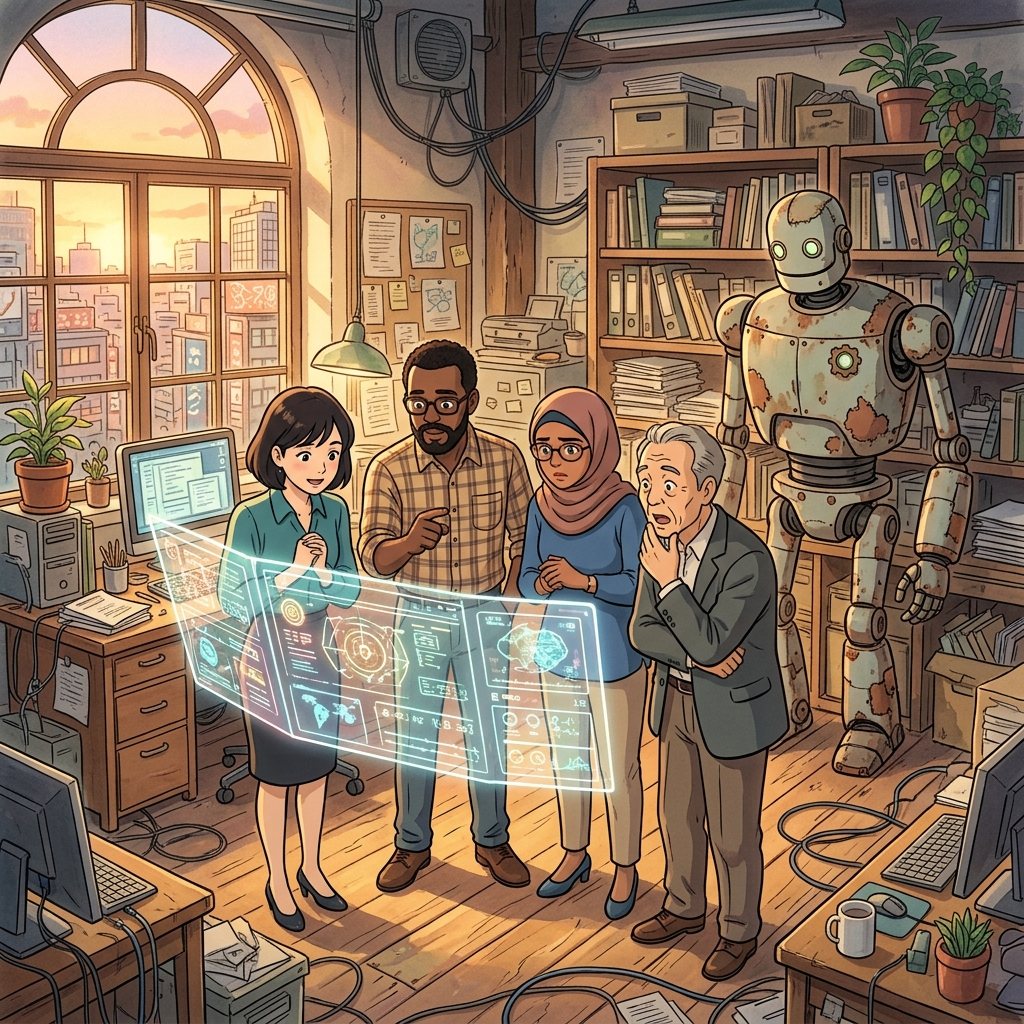
\includegraphics[height=0.6\textheight,keepaspectratio]{Images/ia_amiga_enemiga.png}\caption{IA en el Entorno Laboral}\end{figure}

\end{frame}

\begin{frame}[allowframebreaks,fragile]{Gestión de Riesgos: Privacidad (Ley 1581)}


\begin{itemize}
  \item \textbf{El Error de Novato:} Subir contratos con datos personales a ChatGPT gratuito.
  \item \textbf{El Riesgo Inminente:} Transmisión internacional de datos no autorizada, violación de confidencialidad cliente-abogado.
  \item \textbf{Soluciones Empresariales:} Licencias ``Zero Data Retention'' (Copilot Enterprise, Claude Team, Harvey). Sus datos no entrenan al modelo público.
\end{itemize}
\end{frame}

\begin{frame}[allowframebreaks,fragile]{Bóveda de Privacidad (Visual)}


\begin{figure}\centering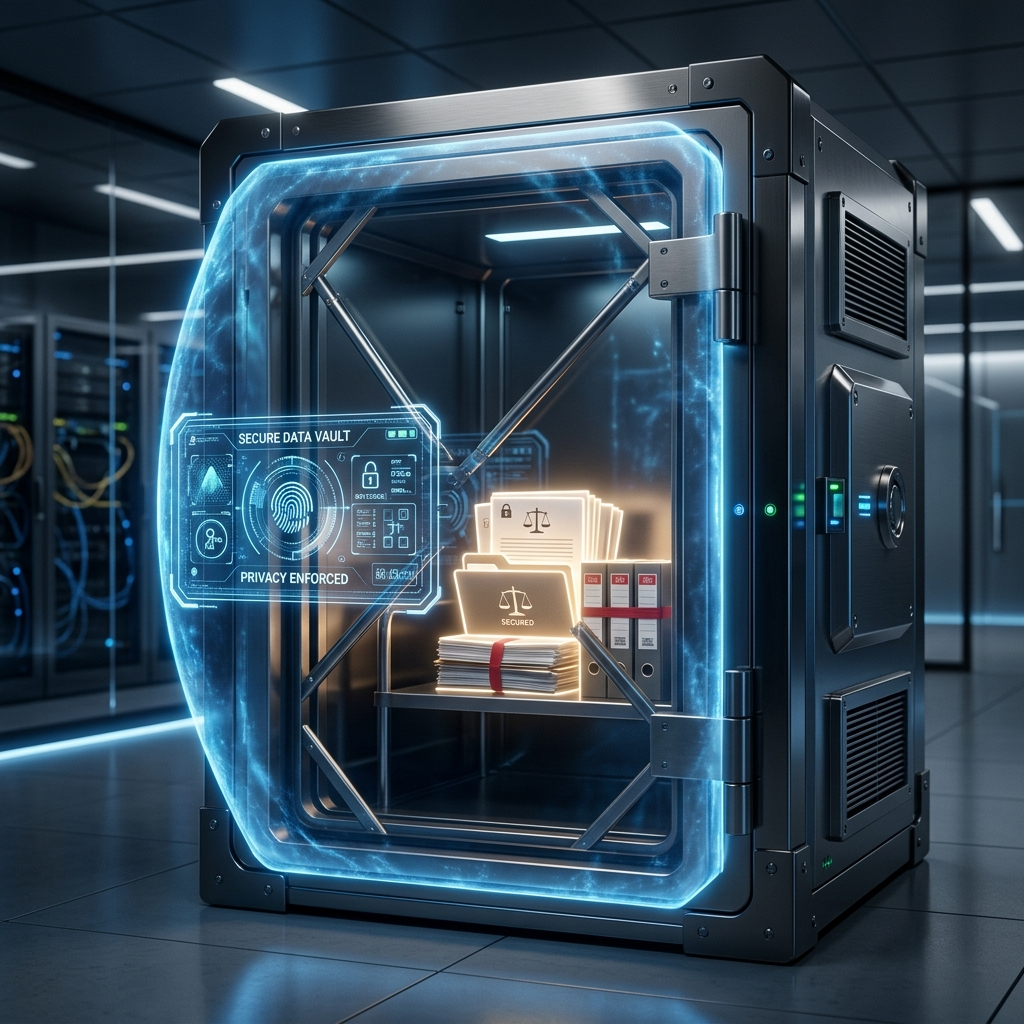
\includegraphics[height=0.6\textheight,keepaspectratio]{Images/privacy_vault_1785900930775.png}\caption{Bóveda de Privacidad Zero Data}\end{figure}

\end{frame}

\begin{frame}[allowframebreaks,fragile]{Privacidad en Herramientas Gratuitas (Opt-Out)}


\textbf{Si su equipo usa cuentas gratuitas, la IA se entrena con sus datos por defecto.} Cómo desactivarlo:

\begin{itemize}
  \item \textbf{ChatGPT:} \textit{Settings} $\rightarrow$ \textit{Data Controls} $\rightarrow$ Apagar \textit{``Improve the model for everyone''}.
  \item \textbf{Claude:} \textit{Settings} $\rightarrow$ \textit{Privacy} $\rightarrow$ Apagar \textit{``Help improve Claude''}.
  \item \textbf{Gemini:} \textit{myactivity.google.com} $\rightarrow$ \textit{Gemini Apps Activity} $\rightarrow$ Seleccionar \textit{``Turn off''}.
\end{itemize}
\textbf{IMPORTANTE - ADVERTENCIA LEGAL (Ley 1581/2012):} Incluso con el \textit{Opt-Out}, subir Datos Personales o Secreto Profesional a entornos B2C gratuitos puede constituir una Transmisión Internacional de Datos no autorizada. La falta de debida diligencia conlleva severas sanciones de la SIC y violaciones a la ética profesional.

\end{frame}

\begin{frame}[allowframebreaks,fragile]{Riesgos: Propiedad Intelectual y 'Alucinaciones'}


\begin{itemize}
  \item \textbf{Derechos de Autor (DNDA):} El producto de la IA no es protegible por derecho de autor sin intervención humana sustancial.
  \item \textbf{Human-in-the-Loop:} La IA no reemplaza la responsabilidad ética y civil del abogado. La supervisión es obligatoria.
\end{itemize}
\end{frame}

\begin{frame}[allowframebreaks,fragile]{Los Desafíos de la IA (Visual)}


\begin{figure}\centering
\includegraphics[height=0.6\textheight,keepaspectratio]{Images/desafios_ia.png}\caption{Desafíos y Auditoría de la IA}\end{figure}

\end{frame}

\begin{frame}[allowframebreaks,fragile]{Taller de Cierre: La Política de IA de su Firma}


\begin{itemize}
  \item \textbf{Actividad en Grupos:} Diseñar los 3 pilares de la política de uso de IA para sus equipos (Qué se permite, qué herramientas, y qué flujos de revisión).
  \item \textbf{Debrief \& Mentoría.}
\end{itemize}
\end{frame}




\end{document}